\section{Introduction} \label{sec:intro}

% Johdatus aihepiiriin (ei liian laajasti, vaan relevantisti ja napakasti)

% Tutkimuskohteen esittely (MITÄ tämä työ tutkii? Kerro työstä/tutkimusaiheesta, ei omasta kirjoitusprosessistasi tai omasta kiinnostuksestasi.)

% Tutkimuksen perustelu: ongelma tai aukko (aiemmassa tutkimuksessa on aukko, tai siitä nousee esiin kysymys, johon tässä etsitään vastausta)

% Tutkimusongelma / -kysymykset (koko työsi sydän, jonka pitäisi näkyä ''punaisena lankana'' koko työn läpi)

% Tavoitteet (Käytä konkreettisesti sanaa ''tavoite'')

% Rajaus (Mitä tämä työ EI tutki)

% Menetelmä, aineisto, teoreettinen kehys (Esittele, MITEN em. aihetta tutkitaan)

%Tulokset? (Johdannossa on ihan hyvä antaa lyhyesti tietoa päätuloksista, mutta ei pakko)

% Työn sisältö ja rakenne (Esittele, miten työn punainen lanka etenee, viittaukset työhön: ``ensin, sitten, seuraavaksi, luvussa 3'' jne.)

\section{Background} \label{sec:background}

\subsection{Video content detection} \label{subsec:detection}

\subsection{Methods} \label{subsec:methods}

\subsection{Validation} \label{subsec:validation}

\section{Research} \label{sec:research}

\subsection{Baseline solution} \label{subsec:baseline}

The simplest method for finding where the closing credits are %of a program begin
is to have a human look at the recording. The accuracy of other methods can be measured by comparing their output to this.
%This creates a reference point for other methods, so that their accuracy can be compared.

Plotting the cumulative user viewing behaviour typically produces a graph that shows a clear pattern, where there is a recess on the beginning and end, and depending on the program, one or a couple recesses in the middle. Checking few recordings by hand, it seems that the recesses match to the non-core-content of the program, that is things before and after the program and ad breaks.

%This is illustrated in figure \ref{fig:intro_ads_outro}.
To illustrate this, the viewer count of a soap opera episode is visualised in figure \ref{fig:intro_ads_outro} with a sample of one hundred viewings. I have checked the beginning and ending timestamps of the intro, ad break and outro. The intro, ad break and outro are highlighted in red on the graph. %in that order.
They match the steep changes in viewer count.

\begin{figure}[H]
\centering
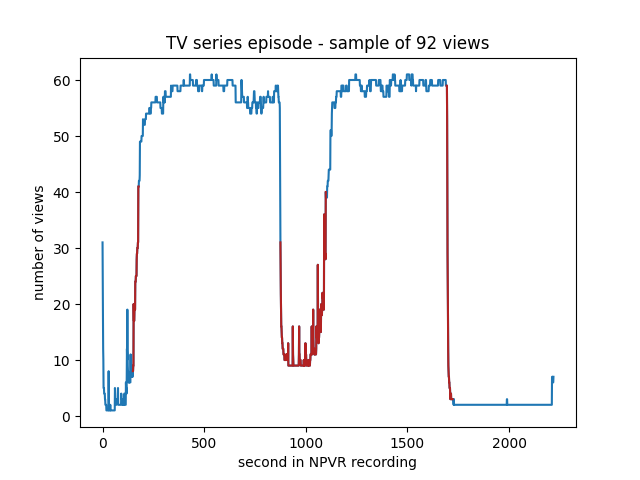
\includegraphics[width=1\textwidth]{../plots/episode.png}
\caption{Example visualisation of user viewer count}
\label{fig:intro_ads_outro}
\end{figure}

\subsection{Dataset} \label{subsec:data}

\subsection{Other solution} \label{subsec:solution}

\section{Results} \label{sec:results}

\section{Conclusions} \label{sec:conclusions}
